\subsection{Basic Properties of Graphene}

Graphene is a two dimensional hexagonal atomic structure (also called honeycomb structure) made of carbon atoms. After its discovery in 2004\cite{novoselov}, graphene has sparked increasing interest among scientists due to its extraordinary mechanical\mcite, optical\mcite and electrical\mcite properties. \note{short summary of properties}

\subsubsection{Graphene Lattice}
\begin{figure}[!h]
  \centering
  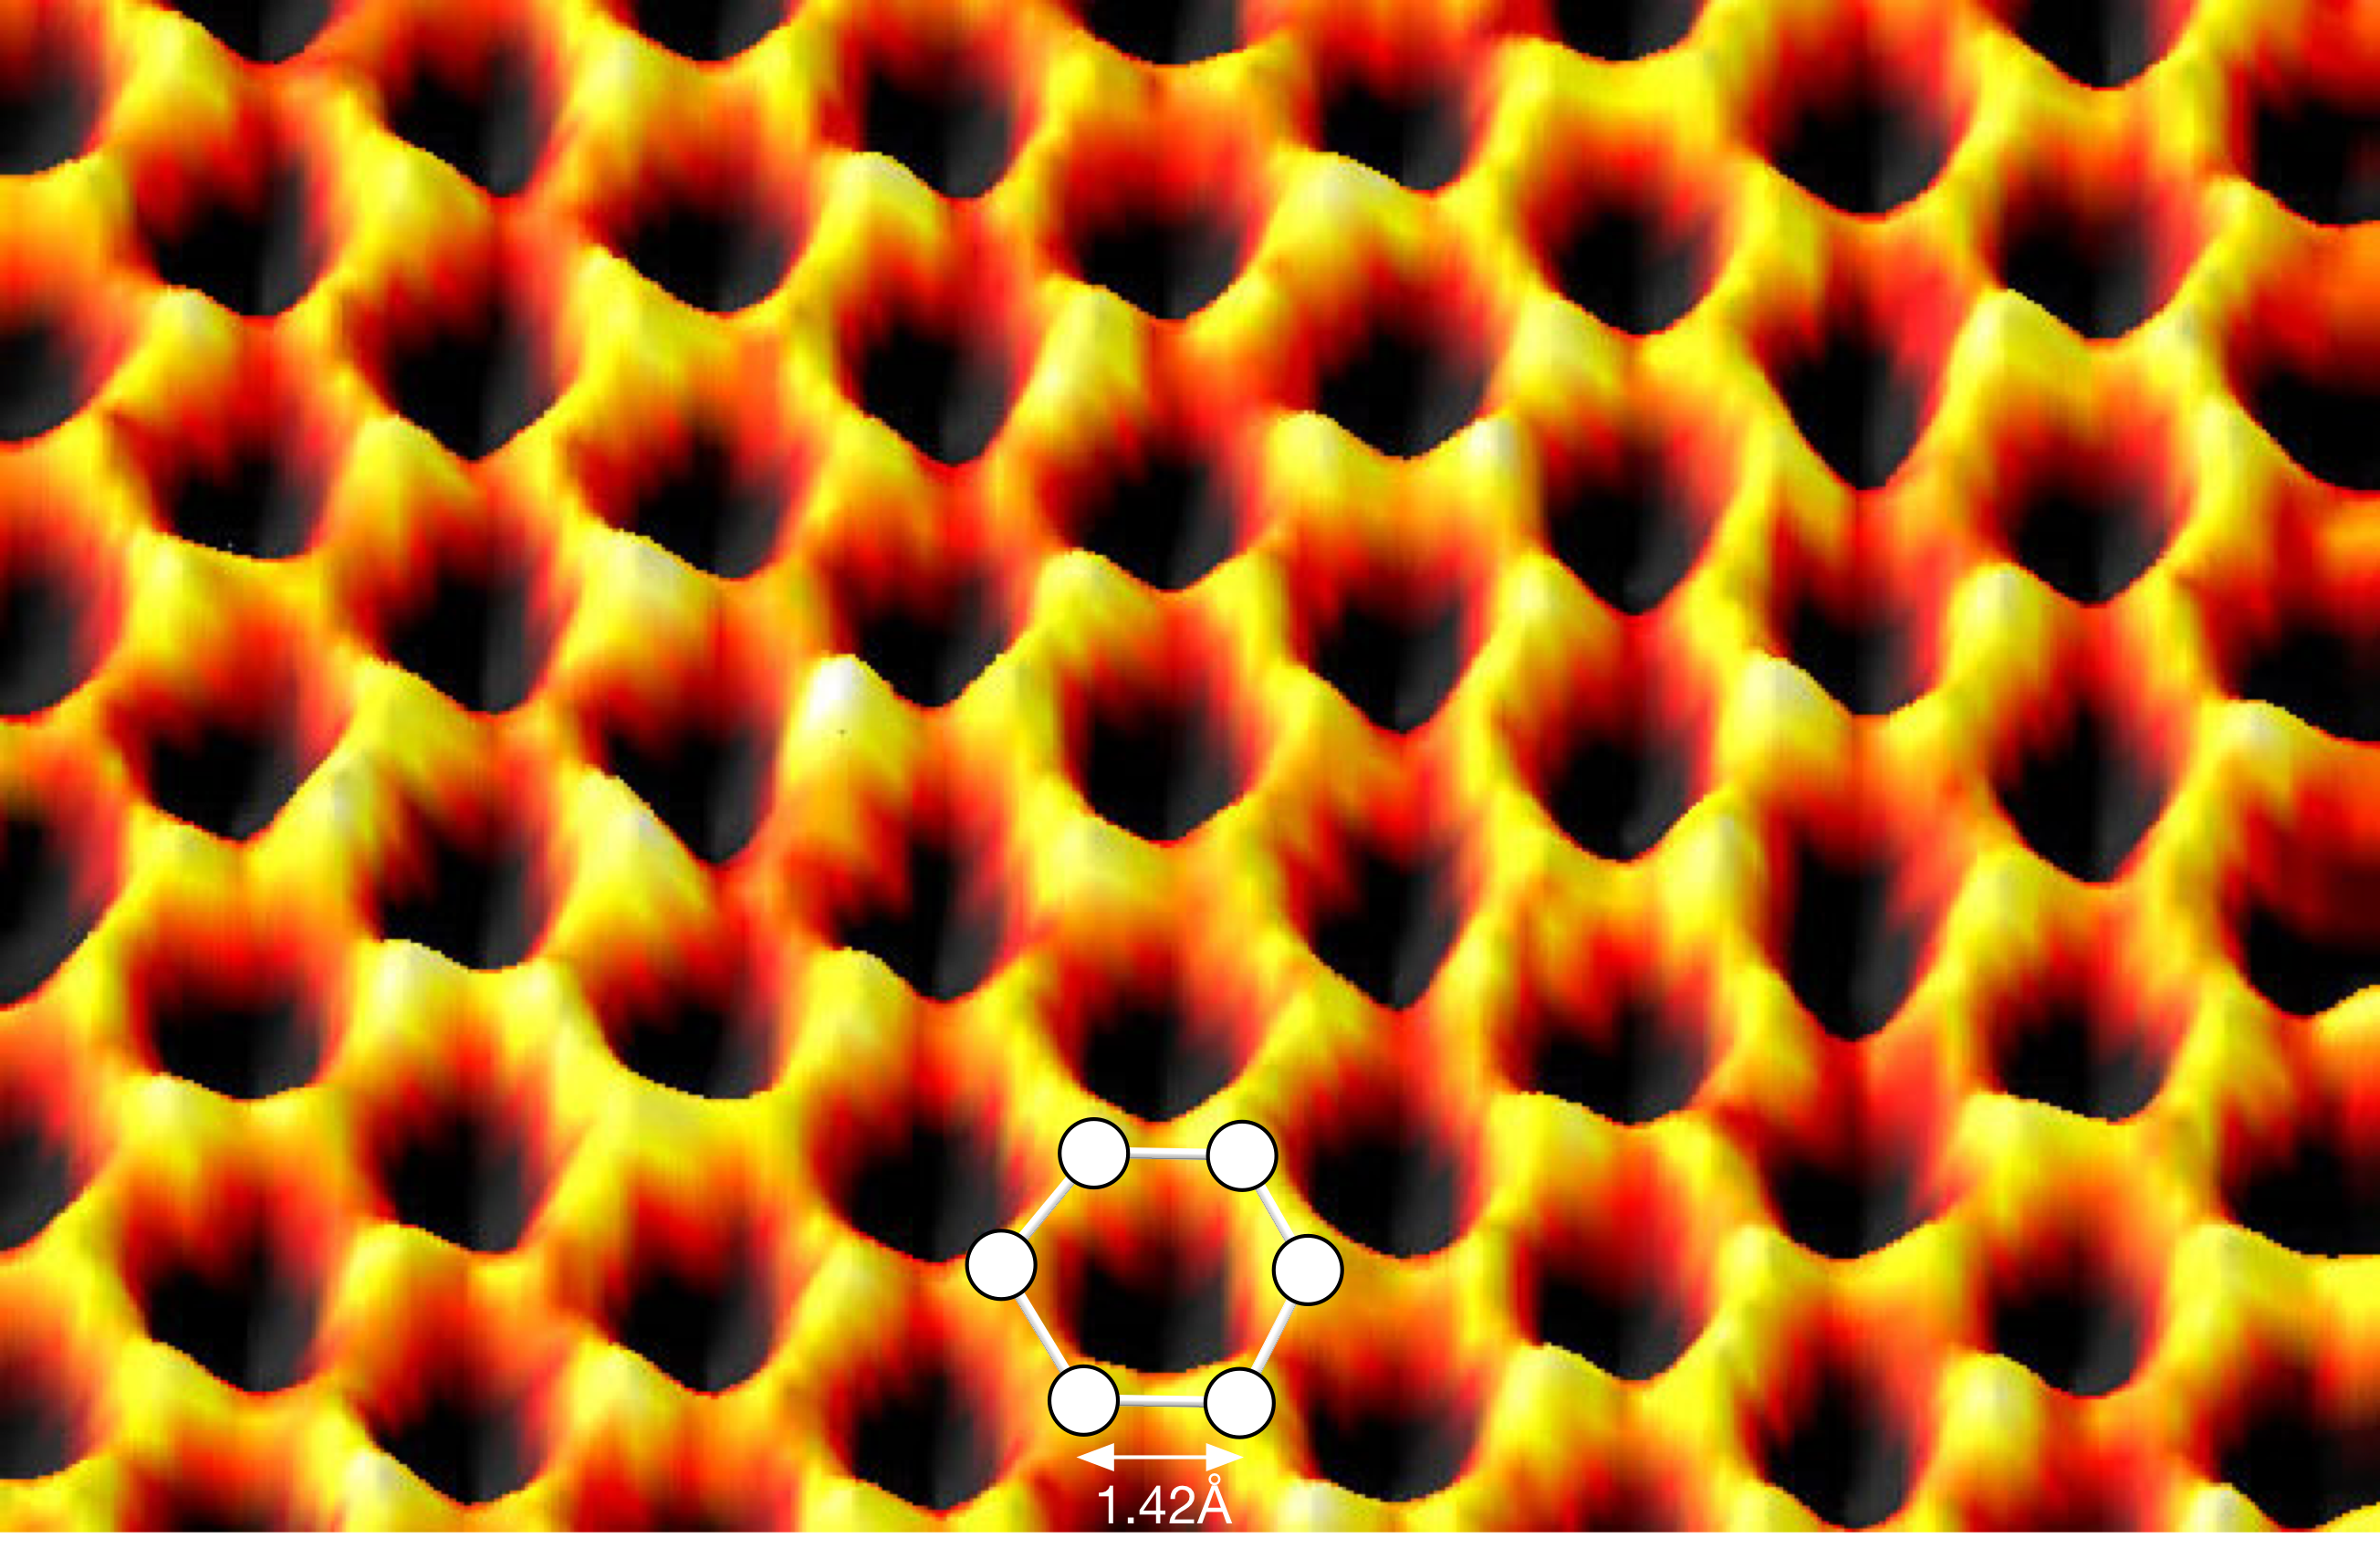
\includegraphics[width=0.7\textwidth]{./images/graphene-spm.png}
  \caption{Graphene's two dimensional hexagonal structure as seen through scanning tunnerling microscopy. The distance between two atoms is about \SI{1.42}{\angstrom} (adapted from \mcite). One hexagon is exemplarily highlighted.}
  \label{fig:spm}
\end{figure}

Graphene is a two dimensional allotrope of carbon where atoms are densely packed in a hexagonal pattern with a distance of about \SI{1.42}{\angstrom} as shown in figure~\ref{fig:spm}. Each sp$^2$-hybridized carbon atom has a covalent $\sigma$-bond to three other carbon atoms.

\begin{figure}[!h]
  \centering
  \begin{subfigure}{0.45\textwidth}
    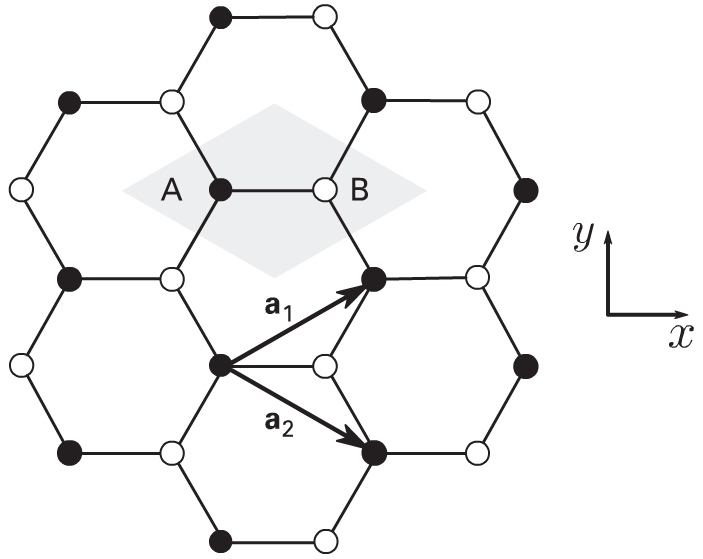
\includegraphics[width=\textwidth]{./images/cell.png}
  \end{subfigure}
  ~
  \begin{subfigure}{0.45\textwidth}
    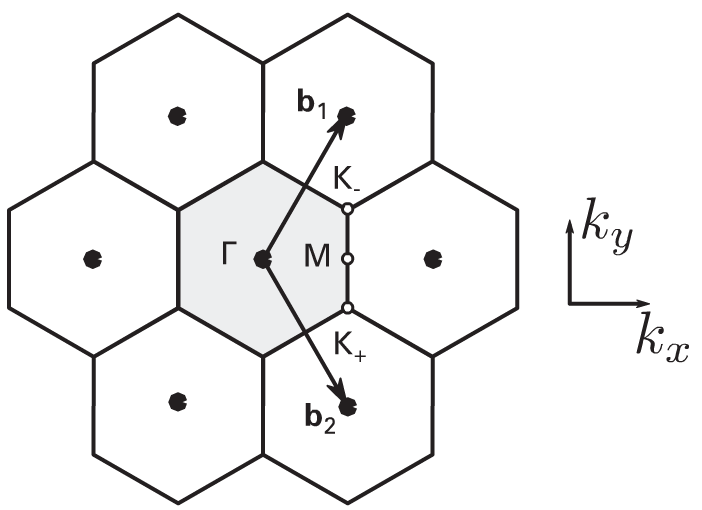
\includegraphics[width=\textwidth]{./images/k-cell.png}
  \end{subfigure}
  \caption{\textbf{(a)} The basis vectors $\mathbf{a}_1$ and $\mathbf{a}_2$ build a triangular Bravais lattice with a two atom-basis. The Wigner-Seitz cell is shaded in gray (adapted from \mcite). \textbf{(b)} The reciprocal lattice points to the hexagonal grid of the two atom base grid. The unit cell is shaded in gray, $\Gamma$ is the cell's center; $K_+$, $K_-$ and $M$ are highly symmetric points (adapted from \mcite). \note{add labels}}
  \label{fig:lattice}
\end{figure}

\begin{figure}[!h]
  \centering
  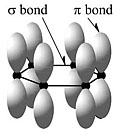
\includegraphics[width=0.3\textwidth]{./images/orbitals.jpg}
  \caption{Valence orbitals of carbon atoms in graphene. Covalent bonded atoms are formed from $\sigma$-orbitals while the perpendicular $\pi$-orbitals create the valence and conduction band. Adapted from http://www.andrew.cmu.edu/user/feenstra/graphene/\mcite.}
  \label{fig:orbitals}
\end{figure}

\subsubsection{Electronic Properties}

The $\pi$ orbitals hybridize and form a delocalized electron cloud above and below the graphene lattice enabling ballistic transport of electrons and a high carrier mobility\mcite.

Due to the symmetry of the system the $\pi$ orbitals can be treated independently as the main contributor to the conduction and valence band. The band structure can be calculated with a tight-binding model as\mcite

\begin{equation}
  E(\mathbf{k})=\pm\sqrt{\gamma_0^2\left(1+4\cos^2\frac{k_ya}{2}+4\cos\frac{k_ya}{2}\cdot\cos\frac{k_x\sqrt{3}a}{2}\right)},
  \label{eq:dispersion}
\end{equation}

with the hopping energy $\gamma_0\approx\SI{2.8}{eV}$, the lattice constant $a\approx\SI{2.46}{Å}$, "$+$" for the conduction band and "$-$" for the valence band.

\begin{figure}[!h]
  \centering
  \begin{subfigure}[b]{0.4\textwidth}
    \caption{}
    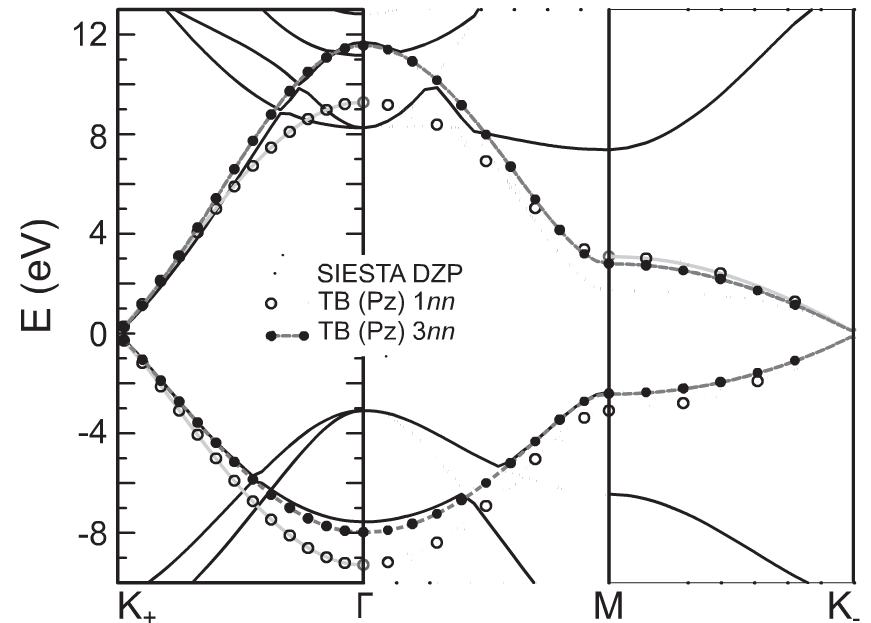
\includegraphics[width=\textwidth]{./images/band-2d.png}
  \end{subfigure}
  ~
  \begin{subfigure}[b]{0.4\textwidth}
    \caption{}
    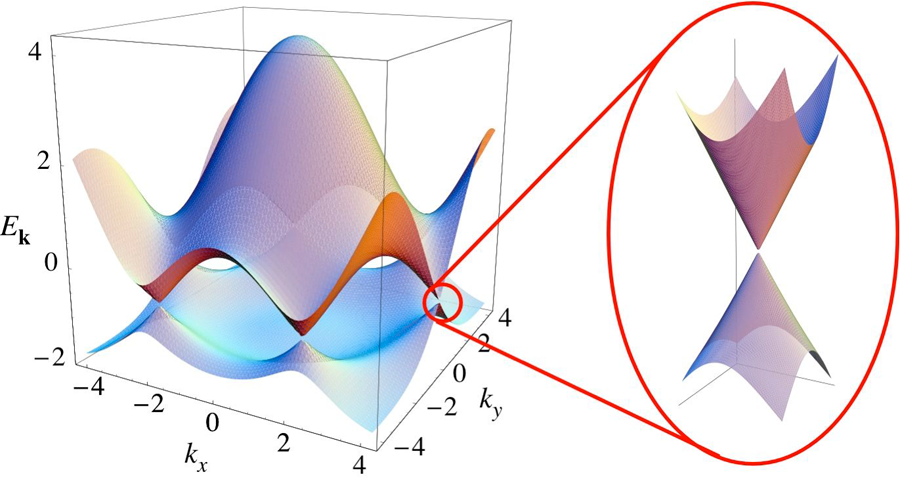
\includegraphics[width=\textwidth]{./images/dispersion.png}
  \end{subfigure}
  \caption { (a): Conduction and valence band touch in the points $K\_-$ and $K\_+$. (b): At the K points the conduction and valance bands can be linearly approximated. }
\end{figure}

Evaluating equation~(\ref{eq:dispersion}) at the K points gives

\begin{equation}
  E(\mathbf{K})=0,
\end{equation}

confirming that conduction and valence band touch in the K points and therefore graphene is a semiconductor without a band gap.

\subsubsection{Other Properties}

Other interesting properties of graphene often exceed those of any other material. It has an intrinsic tensile strength of 130 GPa and a Young's modulus as high as 1TPa\mcite. Also it's impermeable to gases\mcite and has a light absorption of exactly $\pi\alpha$\mcite.
